\documentclass[]{beamer}
%\documentclass[notes]{beamer}       % print frame + notes
%\documentclass[notes=only]{beamer}   % only notes
%\documentclass{beamer}              % only frames
%\documentclass[handout]{beamer}
\usepackage{tikz}
\usepackage{amsmath}
\usepackage{algorithm2e}

\usetheme{Dresden}%%%%% developer's preference - may change based on preferences

%%%%%% UMass official color: https://www.umass.edu/brand/elements/color
\definecolor{UMassAmherst}{rgb}{0.533 0.11 0.11}
\usecolortheme[named=UMassAmherst]{structure}

\title{Grafos}
\author{MSc Edson Ticona Zegarra}
\institute{Campamento de Programaci\'on}
\date{}

%%%%%% obtained from: https://www.umass.edu/brand/elements/wordmarks-seal-and-spirit-marks
%%%%%% logos of other departments can also be obtained from the above link. Otherwise, consult your department website.

\begin{document}

\maketitle

\begin{frame}{Contenido}
\tableofcontents
\end{frame}

\section{Introducci\'on}
\begin{frame}{Contenido}
\tableofcontents[currentsection]
\end{frame}

\begin{frame}{Grafo}
  \begin{itemize}
    \item Un grafo es una estructura de datos definida por un par de conjuntos: los v\'ertices $V$ y las aristas $E$.
      \pause
    \item Toda arista conecta un par de v\'ertices, entonces decimos que $G = (V,E)$
  \end{itemize}
\end{frame}

\begin{frame}{Grafo}
  \centering
  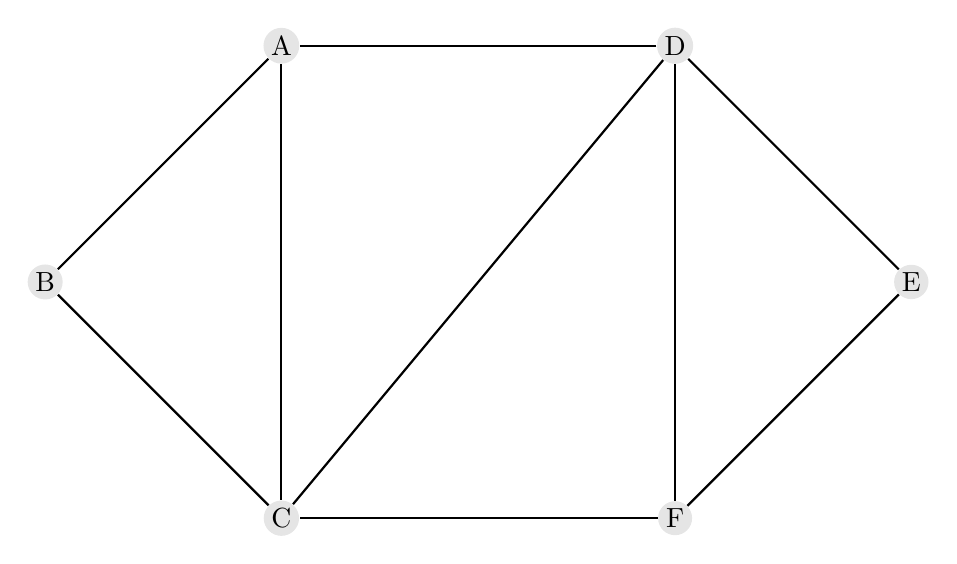
\begin{tikzpicture}
  \tikzstyle{vertex}=[circle,fill=black!10,minimum
  size=12pt,inner sep=1pt]
  \node[vertex](A) at ( 3,3){A};
  \node[vertex](B) at ( 0,0){B};
  \node[vertex](C) at ( 3,-3){C};
  \node[vertex](D) at (8,3){D};
  \node[vertex](E) at (11,0){E};
  \node[vertex](F) at (8,-3){F};
  \path[draw,thick,-] (D) -- (A);
  \path[draw,thick,-] (B) -- (A);
  \path[draw,thick,-] (B) -- (C);
  \path[draw,thick,-] (A) -- (C);
  \path[draw,thick,-] (D) -- (C);
  \path[draw,thick,-] (F) -- (C);
  \path[draw,thick,-] (F) -- (E);
  \path[draw,thick,-] (D) -- (E);
  \path[draw,thick,-] (D) -- (F);
\end{tikzpicture}
\end{frame}

\begin{frame}{Grafo}
  \begin{itemize}
    \item Para el grafo anterior, $V = \{A, B, C, D, E, F\}$
      \pause
    \item $E= \{ (D, A), (B, A), (B, C), (A, C), (D, C), (F, C), (F, E), (D, E), (D, F) \} $
      \pause
    \item formalmente $G=(V,E)$
  \end{itemize}
\end{frame}

\begin{frame}{Grafo}
  \begin{itemize}
    \item Los grafos son \'utiles para representar: redes de comunicaciones, caminos, redes sociales, etc
      \pause
    \item Usualmente consideramos a los grafos como no direccionados, es decir, si existe un v\'ertice $(u,v)$, se puede ir de $u$ a $v$ y viceversa
      \pause
    \item Por otro lado, si consideramos grafos direccionados, gr\'aficamente utilizamos flechas para indicar la direcci\'on y una arista $(u,v)$ indica que se puede ir de $u$ a $v$, pero \textbf{no} de $v$ a $u$. En este caso usualmente utilizamos el t\'ermino \textit{arco} y no arista, as\'i tambi\'en decimos que $G = (V,A)$
      \pause
    \item Entre cualquier par de v\'ertices $u$ y $v$, solo existe a lo mucho una arista para grafos no direccionados. 
      \pause
    \item Para grafos direccionados, para cualquier par de v\'ertices existe a lo mucho una arista $(u,v)$ y una arista $(v,u)$
  \end{itemize}
\end{frame}

\begin{frame}{Grafo}
  \begin{itemize}
    \item Adicionalmente una arista $(u,v)$ puede recibir un \textit{peso}, que puede representar el costo para ir de $u$ a $v$ y se representa por $c_{u,v}$
      \pause
    \item A dichos grafos se les conoce como grafos con pesos
      \pause
    \item Se conoce como grafo \textit{conectado} a todo grafo cuyos v\'ertices tienen al menos un camino entre s\'i
      \pause
    \item Un grafo cuyos v\'ertices representan puntos en el plano se les conocen como grafos geom\'etricos
      \pause
    \item Grafos que contienen m\'as de una arista por par de v\'ertices se le conoce como multi-grafo. Grafos cuyas aristas conectan m\'as de dos v\'ertices se les conocen como hipergrafos.
  \end{itemize}
\end{frame}

\begin{frame}{Multigrafos e Hipergrafos}
  \includegraphics[width=2in]{hypergraph.png}
  \includegraphics[width=2in]{multigraph.png}

  Fuente: Wikimedia. Creative Commons license.
\end{frame}

\begin{frame}{Grafo}
  \begin{itemize}
    \item Un grafo conectado con $|V| - 1 $ aristas es un \'arbol
      \pause
    \item Un \'arbol es un caso particular de un grafo
      \pause
    \item Un grafo que tiene todas las posibles aristas se conoce como grafo \textit{completo}
      \pause
    \item Un grafo es llamado de \textit{denso} si es que $|E| >> |V| $ y es llamado de \textit{esparso} si es que $|E| < |V| $. Esta definici\'on es a veces difusa y depende del problema.
      \pause
    \item Alternativamente, un grafo es esparso si $|E| = O(|V|)$ o $|E| = O(|V| \log |V| )$
  \end{itemize}
\end{frame}

\section{Representaci\'on}
\begin{frame}{Contenido}
\tableofcontents[currentsection]
\end{frame}

\begin{frame}{Lista de adyacencia}
  \begin{itemize}
    \item La representaci\'on b\'asica de un grafo es con una lista de adyacencia o con una matriz de adyacencia
      \pause
    \item Una lista de adyacencia es un vector, con un elemento por v\'ertice $i$. El elemento i-\'esimo almacena a su vez otro vector que contiene la lista de v\'ertices con los cuales el v\'ertice $i$ est\'a conectado
      \pause
    \item Para el grafo mostrado anteriormente, la lista se ver\'a: $G = \{ [D, B, C], [A, C], [B, A, D, F], [A, C, E, F], [D, F], [D, E] \}$
      \pause
    \item Para un grafo con pesos, cada elemento del vector puede contener un par, indicando el v\'ertice al que se conecta la arista y el peso de dicha arista.
      Note que no hay ning\'un \'orden en particular al momento de guardar los v\'ertices
  \end{itemize}
\end{frame}

\begin{frame}{Matriz de adyacencia}
  \begin{itemize}
    \item Una matriz de adyacencia es un matriz, tal que la arista $u,v$ ser\'a representada por un valor de 1 en la fila $u$ y la columna $v$
      \pause
\[
\begin{pmatrix}
  0 & 1 & 1 & 1 & 0 & 0 \\
  1 & 0 & 1 & 0 & 0 & 0 \\
  1 & 1 & 0 & 1 & 0 & 1 \\
  1 & 0 & 1 & 0 & 1 & 1 \\
  0 & 0 & 0 & 1 & 0 & 1 \\
  0 & 0 & 1 & 1 & 1 & 0 \\
\end{pmatrix}
\]
    \pause
    \item Para un grafo con pesos puede guardarse el peso directamente en la matriz. Note que la matriz tiene una diagonal con ceros
      \pause
    \item Un grafo no direccionado tiene una matriz sim\'etrica
  \end{itemize}
\end{frame}

\begin{frame}{Representaciones}
  \begin{itemize}
    \item Est\'as no son las \'unicas maneras de representar un grafo, aunque s\'i las m\'as comunes
      \pause
    \item El uso depende de la situaci\'on, algunos algoritmos o problemas se facilitan con una u otra representaci\'on
      \pause
    \item Para un grafo no direccionado completo, ambas representaciones ser\'an iguales
      \pause
    \item La lista de adyacencia es m\'as eficiente en el uso de memoria
      \pause
    \item Grafos densos son naturalmente mejor representados por una matriz de adyacencia; grafos esparsos por listas de adyacencia
  \end{itemize}
\end{frame}

\section{B\'usqueda en grafos}
\begin{frame}{Contenido}
\tableofcontents[currentsection]
\end{frame}

\begin{frame}{B\'usqueda}
  \begin{itemize}
    \item Es una forma de visitar todos los v\'ertices de un grafo hasta encontrar el valor deseado
      \pause
    \item A diferencia de una arreglo, los grafos pueden ser recorridos de diversas maneras
      \pause
    \item Cada forma tiene sus ventajas y sus aplicaciones
  \end{itemize}
\end{frame}

\subsection{BFS}
\begin{frame}{Breadth First Search (BFS): B\'usqueda en amplitud}
  \begin{itemize}
    \item Se comienza en un v\'ertice $v$ y se avanza como una ``gota de agua'', recorriendo primero los vecinos de $v$, luego los v\'ertices que est\'an a dos saltos de $v$, luego los que est\'an a tres saltos, y as\'i hasta recorrer todo el grafo.
      \pause
    \item La complejidad es $O(|V| + |E|)$
  \end{itemize}
\end{frame}

\begin{frame}{Breadth First Search (BFS): B\'usqueda en amplitud}
  \begin{algorithm}[H]
    %\SetKwInOut{Input}{input}\SetKwInOut{Output}{output}
    %\Input{$G$ es el grafo y $x$ el v\'ertice buscado.}
    %\Output{$0$ si $x \in V$, $1$ caso contrario}
    %\BlankLine
    {$ toVisit.push(u) $} \tcp*{$toVisit$ puede ser una cola y se comienza en un v\'ertice arbitrario $u$}
    \While{$ !toVisit.empty() $}
    {
      $u = toVisit.front() $
      \tcc{$Adj(u)$ adyacentes a $u$}
      \For{$v \in Adj(u)$}
      {
        \tcc{colorear los v\'ertices}
        \If{$ !visited(v) $}
        {
          {$ toVisit.push(v)  $} \;
          { dist[v] = dist [u] + 1 } \;
          { mark $u$ as visited } \;
        }
      }
      { $toVisit.pop()$ }
    }
  \end{algorithm}
\end{frame}

\begin{frame}{Breadth First Search (BFS): B\'usqueda en amplitud}
  \begin{itemize}
    \item ?`Qu\'e pasa si el grafo no esta conectado?
      \pause
    \item ?`C\'omo hallar la distancia m\'inima entre dos v\'ertices para un grafo sin pesos?
  \end{itemize}
\end{frame}

\subsection{DFS}
\begin{frame}{Depth First Search (DFS): B\'usqueda en profundidad}
  \begin{itemize}
    \item Se comienza desde un v\'ertice $v$ y se trata de llegar lo m\'as lejos posible en n\'umero de saltos, luego se regresa hasta el \'ultimo nodo visitado que tenga vecinos a\'un sin visitar, y se vuelve a intentar llegar lo m\'as lejos posible en n\'umero de saltos hasta recorrer todo el grafo.
      \pause
    \item La complejidad es $O(|V| + |E|)$
  \end{itemize}
\end{frame}

\begin{frame}{Depth First Search (DFS): B\'usqueda en profundidad}
  \begin{algorithm}[H]
    %\SetKwInOut{Input}{input}\SetKwInOut{Output}{output}
    %\Input{$A$ es un conjunto de $n$ n\'umeros y $x$ es el n\'umero buscado.}
    %\Output{$0$ si $x \in A$, $1$ caso contrario}
    %\BlankLine
    mark $u$ as visited \;
    \For{$v \in Adj(u)$}
    {
      \If{$ !visited(v) $}
      {
        $ DFS(v) $
      }
    }
  \end{algorithm}
\end{frame}

\begin{frame}{Depth First Search (DFS): B\'usqueda en profundidad}
  \begin{itemize}
    \item ?`Qu\'e pasa si el grafo no esta conectado?
      \pause
    \item ?`C\'omo podr\'iamos hacer el ordenamiento topol\'ogico en un grafo direccionado?
      \pause
    \item ?`C\'omo hallamos los componentes fuertemente conectados para un grafo direccionado?
  \end{itemize}
\end{frame}

\end{document}
